%!TEX root = widefieldscan.tex
\svnidlong
{$HeadURL$}
{$LastChangedDate$}
{$LastChangedRevision$}
{$LastChangedBy$}
\framebox{Author: \svnauthor|Rev: \svnrev|Last change: \svndate}% - URL: \url{\svnkw{HeadURL}}}
\section{Materials and Methods}
\label{sec:materials and methods}
\subsection{Animal Handling and Tissue Preparation}
The preparation of the lung samples has been performed according to~\citet{Schittny1997,Schittny1998}. Briefly, the lungs have been extracted from Sprague-Dawley rats after they have been perfused and filled with phosphate buffered saline by instillation via tracheostomy until the midrespiratory lung volume was reached.

The extracted lung lobes have been fixed for potential storage in 2.5\% glutaraldehyde (C$_5$H$_8$O$_2$). For the preparation of the imaging the samples have been postfixed---as in electron microscopy---with 1\% osmium tetroxide (OsO$_4$) and stained with 4\% uranyl acetate (C$_4$H$_6$O$_6$U), dehydrated in a graded series of ethanol and transferred into paraffin. \todo{Citation needed! Or longer explanation} Osmium tetroxide and uranyl acetate exhibit a higher absorption contrast for x-rays than the unstained lung tissue, thus facilitating the imaging of the stained tissue. The lung samples have been mounted onto standard electron microscopy sample mounts with a diameter of approximately \SI{13}{\milli\meter} (PLANO GmbH, Wetzlar, Germany) using paraffin.

Handling of the animals before and during the experiments, as well as the experiments themselves, were approved and supervised by the Swiss Agency for the Environment, Forests and Landscape and the Veterinary Service of the Canton of Bern.

\subsection{SRXTM}
The experiments were performed on the TOMCAT beamline at the Swiss Light Source, Paul Scherrer Institut, Villigen, Switzerland. TOMCAT is one of 15 currently operating beam lines at the SLS. TOMCAT is located at the port X02DA of the SLS. The beamline receives photons from a \SI{2.9}{\tesla} super-bending magnet. The critical energy of this super-bending magnet is \SI{11.1}{\kilo\electronvolt} (corresponding to a wavelength of \SI{0.122}{\nano\meter}). Detailed technical specifications of the beamline and beam characteristics have been described by~\citet{Stampanoni2006a,Stampanoni2007}.

\subsubsection{Image Acquisition}
The sample holder at TOMCAT is equipped with an appropriate collet chuck to mount standard electron microscopy (EM) sample tables into the beam. The samples have been scanned at an x-ray energy of \SI{12.6}{\kilo\electronvolt}. After penetration of the sample, the x-rays are converted into visible light by a Ce-doped YAG scintillator (Crismatec Saint-Gobain, Nemours, France). The projection images were further magnified by diffraction limited microscope optics and digitized by a high-resolution 2048$\times$2048 pixel CCD camera. All samples were imaged using a 10$\times$ magnification, with 2$\times$2 binning and \SI{125}{\milli\second} exposure time or no binning and \SI{500}{\milli\second} exposure time, resulting in isotropic voxels of a side length of \SI{1.4}{\micro\meter} or of \SI{0.70}{\micro\meter} \todo{correct voxel side length?}, respectively.

As mentioned in section~\ref{subsec:enhancing the field of view}, to obtain an enhanced FOV, we need to scan the samples with multiple subscans at varying positions covering the whole sample. To achieve this, we have written a custom MATLAB-script \todo{Script(s) in Appendix?}(MATLAB$^\text{\textregistered}$ 7.6.0.321 (R2008a), The MathWorks, Inc.), where the user is able to input the scanning parameters like desired FOV, detector width, desired overlap between the subscans, magnification and binning. The script then simulates different scanning protocols and calculates the expected reconstruction quality, which is then plotted against the acquisition time. Such a plot is shown in figure~\ref{fig:2008c-qualityplot}.

\begin{figure}
	\centering
		%\documentclass{article}
%\usepackage{tikz,pgfplots}
%\usepackage[pdftex,active,tightpage]{preview}
%\begin{document}
%\begin{preview}
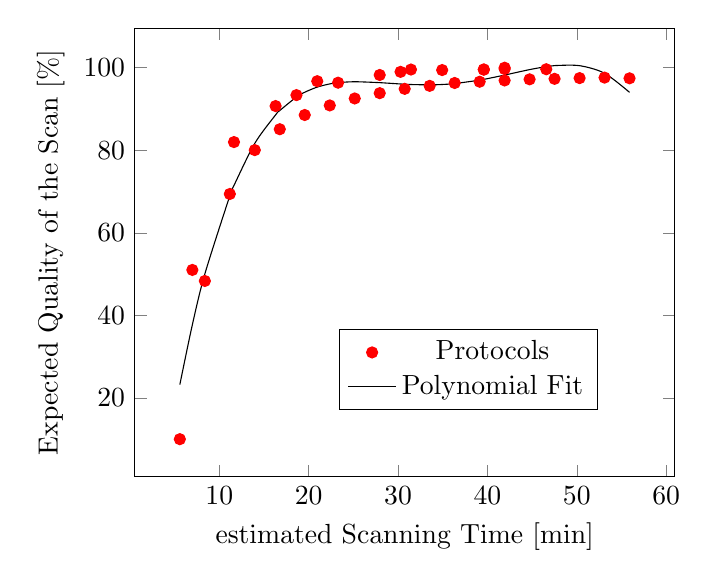
\begin{tikzpicture}
\begin{axis}[%
%	width=\linewidth,%
	xlabel={estimated Scanning Time [min]},%
	ylabel={Expected Quality of the Scan [\%]},%
	]

% Line plot
\addplot [ color = red, only marks, mark = *] 
coordinates{
 (5.5875,10) (6.98958,51.0063) (8.3875,48.3324) (11.1813,69.4075) (11.6458,81.985) (13.975,80.0399) (16.3021,90.7093) (16.7688,85.096) (18.6354,93.3621) (19.5625,88.5423) (20.9625,96.7319) (22.3625,90.8617) (23.2917,96.3704) (25.1563,92.5481) (27.9479,98.2413) (27.95,93.8354) (30.2813,98.9979) (30.7437,94.8773) (31.4438,99.5581) (33.5375,95.6051) (34.9375,99.4314) (36.3375,96.2983) (39.1313,96.6062) (39.5938,99.5875) (39.5958,99.5241) (41.925,100) (41.925,96.9138) (41.9271,99.6929) (44.7188,97.1848) (46.5833,99.6309) (47.5125,97.3067) (50.3125,97.4836) (53.1063,97.603) (55.9,97.4336)
};

% Line plot
\addplot [ smooth ] 
coordinates{
 (5.5875,23.213) (6.98958,37.7379) (8.3875,50.0404) (11.1813,68.9695) (11.6458,71.4736) (13.975,81.6837) (16.3021,88.5733) (16.7688,89.6234) (18.6354,92.9028) (19.5625,94.0559) (20.9625,95.3079) (22.3625,96.078) (23.2917,96.3777) (25.1563,96.6032) (27.9479,96.3862) (27.95,96.3859) (30.2813,96.0569) (30.7437,96.0006) (31.4438,95.9286) (33.5375,95.8484) (34.9375,95.9383) (36.3375,96.1591) (39.1313,96.986) (39.5938,97.167) (39.5958,97.1679) (41.925,98.211) (41.925,98.211) (41.9271,98.212) (44.7188,99.5426) (46.5833,100.268) (47.5125,100.516) (50.3125,100.492) (53.1063,98.6574) (55.9,94.0299)
};

\pgfplotsset{every axis legend/.append style={
at={(0.618,0.2)},
anchor=base}}

\legend{Protocols,Polynomial Fit}%$p(x)=p_{1}x^{n}+p_{2}x^{n-1}+...+p_{n}x+p_{n+1}$}

\end{axis}
\end{tikzpicture}
%\end{preview}
%\end{document}
	\caption{Quality-Plot of 34 calculated protocols. The red dots show the expected the quality of the, the black plot is a polynomial fit $p$p with $x=4$ for $p(x)=p_{1}x^{n}+p_{2}x^{n-1}+...+p_{n}x+p_{n+1}$. 19 of these protocols have been scanned. Details of these scans are shown in table~\ref{tab:projections} and are discussed in section~\ref{sec: Results I}.}
	\label{fig:2008c-qualityplot}
\end{figure}

The proposed protocols are designed in such a way that the total scanning time---which scales with the total amount of recorded projections---can be greatly reduced. Depending on the demand of the end-user, we were able to reduce the total acquisition time by 86\percent, as can be seen in table~\ref{tab:projections}. Albeit this reduction introduces some artifacts in the dataset, an automated segmentation of the airways is still possible, as is shown later on. \todo{show this segmentation lateron!}


\begin{table}[tb]
\centering
	\caption{Specification of different protocols and time used compared to gold standard}
	\begin{tabular*}{\textwidth}{l@{\extracolsep\fill}ccccccccccccccccccc}
		\toprule
		Protocol 			& B & C & D & E & F & G & H\\
		\midrule
		Total Projections 	& 15732 & 13110 & 13110 & 10925 & 11799 & 9833 & 10488\\
		Time [\%] 			& 100 & 83.33 & 83.33 & 69.44 & 75 & 62.5 & 66.67\\
%		\bottomrule
	\end{tabular*}
	\begin{tabular*}{\textwidth}{l@{\extracolsep\fill}ccccccccccccccccccc}
		\toprule
		Protocol 			& I & J & K & L & M & N \\
		\midrule
		Total Projections 	& 5436 & 8740 & 9177 & 7648 & 7866 & 6555 \\
		Time [\%] 			& 34.7 & 55.6 & 58.3 & 48.6 & 50 & 41.7 \\
%		\bottomrule
	\end{tabular*}
	\begin{tabular*}{\textwidth}{l@{\extracolsep\fill}ccccccccccccccccccc}
		\toprule
		Protocol 			& O & P & Q & R & S & T \\
		\midrule
		Total Projections 	& 6555 & 5244 & 4370 & 3933 & 2622 & 2185 \\
		Time [\%] 			& 41.7 & 33.3 & 27.8 & 25 & 16.7 & 13.9 \\
		\bottomrule
	\end{tabular*}
	\label{tab:projections}
\end{table}

After the user has chosen a suitable protocol, the MATLAB-script writes a preference file to the disk, which is then parsed by a custom Python-script used for the interaction with the EPIC-System (Experimental Physics and Industrial Control System, \url{http://www.aps.anl.gov/epics/}), which is then operating the TOMCAT beamline without user intevention. All parameters like filename, sample-position in relation to the beam, rotation angles and amount of projections to obtain for the subscans have been set beforehand by the MATLAB-script, read out by the Python-script so that all the scans could be performed as a batch job without manual intervention. The sample on the sample holder was thus not touched during the acquisition of the different subscans. 

\subsection{Image Processing}
\label{subsec:image processing}
After the acquisition of the sub-scan projection images, these image sets are corrected with the so called dark field and flat field images. The dark field images are obtained while all the shutters are closed---thus no x-rays are present---and are used for the detection of camera noise and dark current. The flat field images (FI) are obtained with x-ray beam, but without the sample. They are recorded to remove the varying beam profile brightness from the projection images. The projections (PI) are first baseline corrected, then the average of the dark images is subtracted and afterwards they are normalized into corrected projections (CPR) as seen in equation~\ref{eq:correction}:%
\begin{equation}
	\text{CPR}=-ln\left(\frac{\text{PI}}{\text{FI}}\right)=ln(\text{FI})-ln(\text{PI})
	\label{eq:correction}
\end{equation}

\subsubsection{Stitching}
\label{subsec:stitching}
Generally, tomographic images are obtained in such a manner, that the sample is rotated for \SI{180}{\degree} while several projection images---essentially single radiographies---are obtained, as is shown in figure~\ref{fig:covering-one scan}. After reconstructing the sample, the images show the FOV of the camera.

\begin{figure*}[tb]
	\centering
	\subfloat[\SI{180}{\degree}]{%\documentclass{article}
%\usepackage[pdftex,active,tightpage]{preview}
%\usepackage{tikz}
%\usepackage{pgfplots}
%\usetikzlibrary{plotmarks}
%\begin{document}
%\begin{preview}
	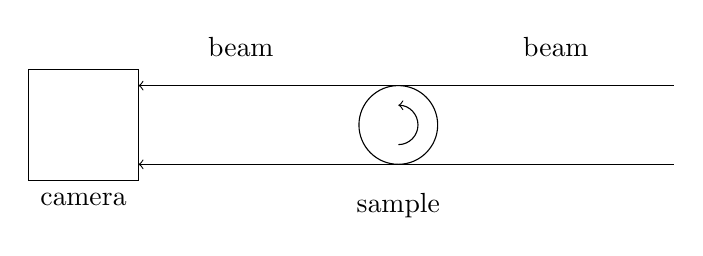
\begin{tikzpicture}
		%drawing grid
		%\draw[color=gray] (0,0) grid (8,1);
		%camera
		\draw (-.2,-.2) rectangle (1.2,1.2);
		\draw (.5,-.25) node [below] {camera};
		% beam
		\draw[<-] (1.2,0) -- (8,0);
		\draw[<-] (1.2,1) -- (8,1);
		\draw (2.5,1.25) node [above] {beam};
		\draw (6.5,1.25) node [above] {beam};
		%sample
		\draw (4.5,0.5) circle (.5);
		\draw (4.5,-.25) node [below] {sample};
		%sample rotation
		\draw[->] (4.5,0.25) arc (-90:90:.25);
	\end{tikzpicture}
%\end{preview}
%\end{document}\label{subfig:cover180}}\\
	\subfloat[\SI{360}{\degree}]{%\documentclass{article}
%\usepackage[pdftex,active,tightpage]{preview}
%\usepackage{tikz}
%\usepackage{pgfplots}
%\usetikzlibrary{plotmarks}
%\begin{document}
%\begin{preview}
	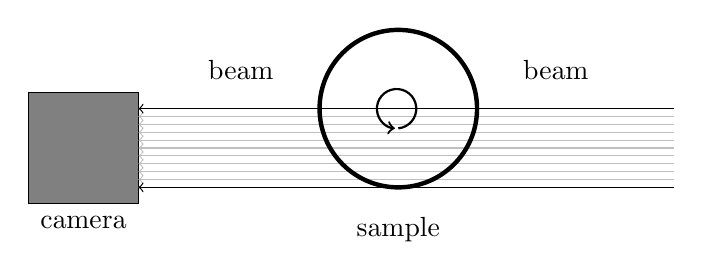
\begin{tikzpicture}
		%drawing grid
		%\draw[color=gray] (0,0) grid (8,1);
		%camera
		\draw[fill=gray] (-.2,-.2) rectangle (1.2,1.2);
		\draw (.5,-.25) node [below] {camera};
		% beam
		\foreach \x in {0,...,10}
			\draw[gray!50,<-] (1.2,0.1*\x) -- (8,0.1*\x);
		\draw[<-] (1.2,0) -- (8,0);
		\draw[<-] (1.2,1) -- (8,1);			
		\draw (2.5,1.25) node [above] {beam};
		\draw (6.5,1.25) node [above] {beam};
		%sample
		\draw[ultra thick] (4.5,1) circle (1);
		\draw (4.5,-.25) node [below] {sample};
		%sample rotation
		\draw[thick,->] (4.5,0.75) arc (-85:265:.25);
	\end{tikzpicture}
%\end{preview}
%\end{document}\label{subfig:cover360}}
	\caption{Covering the FOV -- one scan}
	\label{fig:covering-one scan}
\end{figure*}

\begin{figure*}[tb]
	\centering
		\documentclass{article}
\usepackage[pdftex,active,tightpage]{preview}
\usepackage{tikz}
\usetikzlibrary{arrows,shapes,backgrounds}
\begin{document}
\begin{preview}
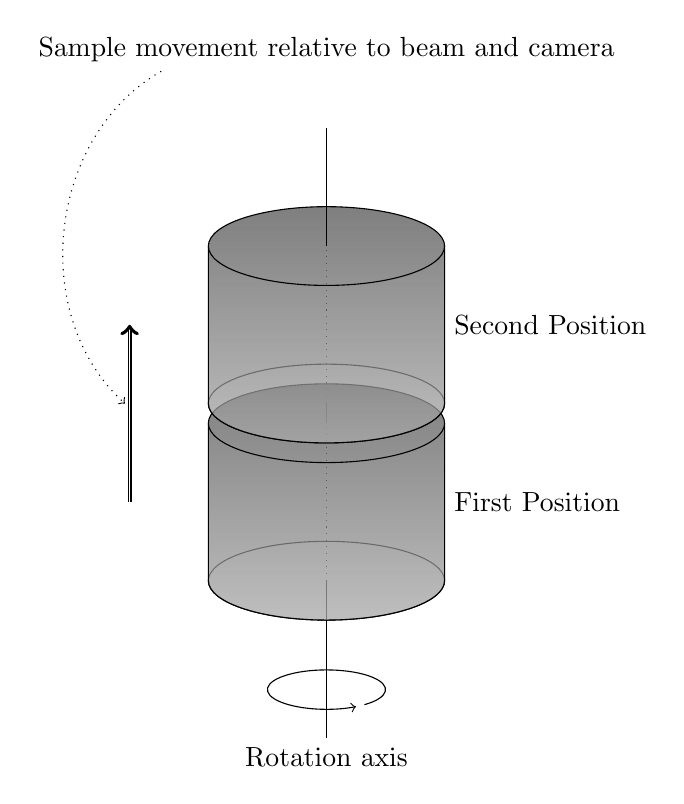
\begin{tikzpicture}%[ultra thick,scale=1]%,show background grid]
	%draw axes
		%\draw[ultra thick] (-10,0) -- (10,0);
		%\draw[ultra thick] (0,-10) -- (0,10);
		%\draw[ultra thick] (0,0) circle (.125);
	% rotation axis
		\draw[->] (0,-2) ++ (-50:.75) arc (-50:300:.75 and .25);
		\draw (0,-3) node [below] {Rotation axis} -- ++(0,2);
		\draw[dotted] (0,-1) -- ++(0,2);
		\draw (0,1) -- ++(0,0.25);
		\draw[dotted] (0,1.25) -- ++(0,2);
	% position 1
		\draw (0,-1) circle (1.5 and .5);
		\fill[shade,semitransparent] (-1.5,-1) arc (-180:0:1.5 and .5) -- ++(0,2) arc (0:180:1.5 and .5) -- cycle;
		\draw (-1.5,-1) arc (-180:0:1.5 and .5) -- ++(0,2) arc (0:180:1.5 and .5) -- cycle;		
		\draw (-1.5,1) arc (-180:0:1.5 and .5);
		\draw (1.5,0) node [right] {First Position};
	% position 2
		\draw (0,1.25) circle (1.5 and .5);
		\fill[shade,semitransparent] (-1.5,1.25) arc (-180:0:1.5 and .5) -- ++(0,2) arc (0:180:1.5 and .5) -- cycle;
		\draw (-1.5,1.25) arc (-180:0:1.5 and .5) -- ++(0,2) arc (0:180:1.5 and .5) -- cycle;		
		\draw (-1.5,3.25) arc (-180:0:1.5 and .5);
		\draw (1.5,2.25) node [right] {Second Position};
	% rotation axis on top
		\draw (0,3.25) -- ++(0,1.5);									
	% sample movement
		\draw[double,->] (-2.5,0) -- (-2.5,2.25) ;% node [text width=10cm,midway,left] {Sample movement relative to beam and camera};	
		% sample movement
		\node (movefrom) at (0,5.75) {Sample movement relative to beam and camera};
		\node (moveto) at (-2.5,1.125) {};
		\draw [->,dotted] (movefrom) to [bend right=54] (moveto);
\end{tikzpicture}
\end{preview}
\end{document}
	\caption{Stacked Scanning - long and thin samples}
	\label{fig:stacked-scanning}
\end{figure*}

\begin{figure*}[tb]
	\centering
		%\documentclass{article}
%\usepackage[pdftex,active,tightpage]{preview}
%\usepackage{tikz}
%\begin{document}
%\begin{preview}
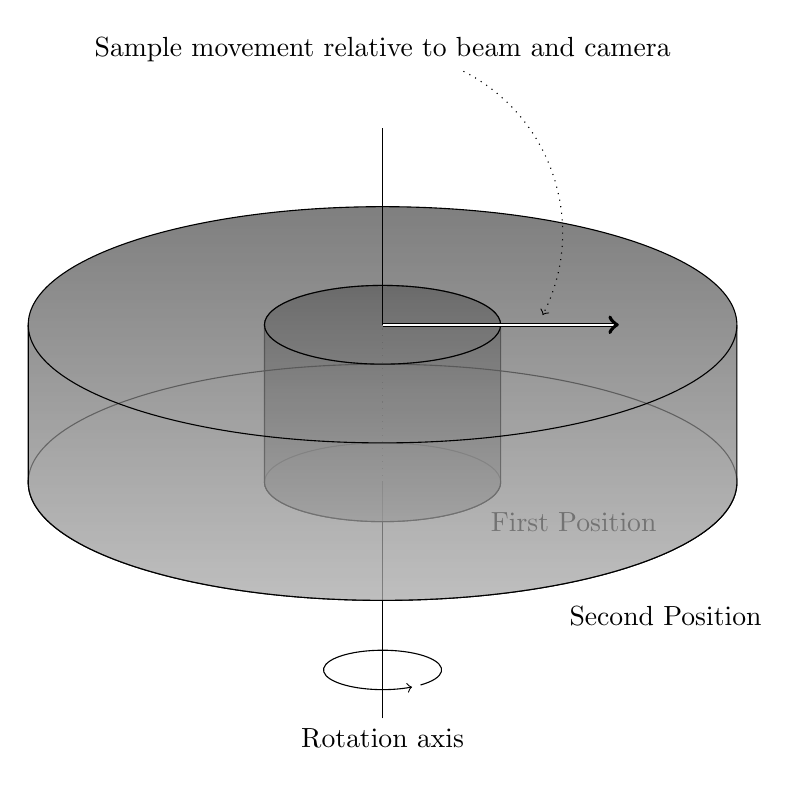
\begin{tikzpicture}%[ultra thick,scale=1]%,show background grid]
	%draw axes
		%\draw[ultra thick] (-10,0) -- (10,0);
		%\draw[ultra thick] (0,-10) -- (0,10);
		%\draw[ultra thick] (0,0) circle (.125);
	% rotation axis
		\draw[->] (0,-3) ++ (-50:.75) arc (-50:300:.75 and .25);
		\draw[] (0,-4) node [below] {Rotation axis} -- ++(0,3);
		\draw[dotted] (0,-1) -- ++(0,2);
	% position 1
		\draw (0,-1) circle (1.5 and .5);
		\fill[shade,semitransparent] (-1.5,-1) arc (-180:0:1.5 and .5) -- ++(0,2) arc (0:180:1.5 and .5) -- cycle;
		\draw (-1.5,-1) arc (-180:0:1.5 and .5) -- ++(0,2) arc (0:180:1.5 and .5) -- cycle;		
		\draw (-1.5,1) arc (-180:0:1.5 and .5);
		\draw (1.25,-1.5) node [right] {First Position};
	% position 2
		\draw (0,-1) circle (4.5 and 1.5);
		\fill[shade,semitransparent] (-4.5,-1) arc (-180:0:4.5 and 1.5) -- ++(0,2) arc (0:180:4.5 and 1.5) -- cycle;
		\draw (-4.5,-1) arc (-180:0:4.5 and 1.5) -- ++(0,2) arc (0:180:4.5 and 1.5) -- cycle;		
		\draw (-4.5,1) arc (-180:0:4.5 and 1.5);
		\draw (2.25,-2.7) node [right] {Second Position};
	% top from position 1 on top
		\draw (0,1) circle (1.5 and .5);
	% rotation axis on top
		\draw (0,1) -- ++(0,2.5);									
	% sample movement
		\draw[double,->] (0,1) -- (3,1);
		\node (movefrom) at (0,4.5) {Sample movement relative to beam and camera};
		\node (moveto) at (2,1) {};
		\draw [->,dotted] (movefrom) to [bend left=45] (moveto);
\end{tikzpicture}
%\end{preview}
%\end{document}
	\caption{Stacked Scanning - broad samples}
	\label{fig:widefield-scanning}
\end{figure*}

If we want to achieve tomographic scans covering a broader FOV, we have to move the sample in relation to the beam and camera, to be able to record projection images from the lateral parts of the sample. This can be done as shown in figure~\ref{fig:covering-three scans a}, \todo{which image variant: \ref{fig:covering-three scans a} or \ref{fig:covering-three scans b}?} where we obtain three subscans to be able to reconstruct a FOV covering the whole sample.

\begin{figure*}[tb]
	\centering
	%\documentclass{article}
%\usepackage[pdftex,active,tightpage]{preview}
%\usepackage{tikz}
%\usepackage{pgfplots}
%\usetikzlibrary{plotmarks}
%\begin{document}
%\begin{preview}
	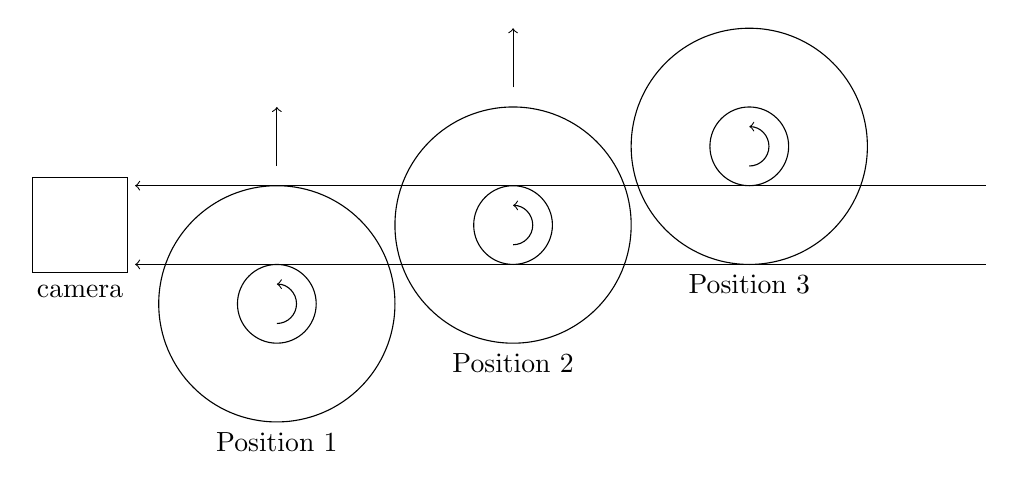
\begin{tikzpicture}[scale=1]
		%drawing grid
%		\draw[color=gray] (0,0) grid (10,1);
		%camera
			\draw (-.1,-.1) rectangle (1.1,1.1);
			\draw (.5,-.35) node {camera};
		% sample positions
			\foreach \x in {1,2,3}{
				\draw     (3*\x,\x-1.5) circle (.5) circle (1.5);			
				\draw[->] (3*\x,\x-1.75) arc (-90:90:.25);
				\draw     (3*\x,-3.25+\x)node {Position \x};
				}
		% movement		
			\foreach \x in {1,2}{				
			    \draw[->]  (3*\x,0.25+\x) -- (3*\x,1+\x);
		% beam
				\draw[<-] (1.2,\x-1) -- (12,\x-1);
				}
	\end{tikzpicture}
%\end{preview}
%\end{document}
	\caption{Covering the FOV -- three scans $\rightarrow$ sample has to move, explain that we still only do \SI{180}{\degree} scans!}
	\label{fig:covering-three scans a}
\end{figure*}

\begin{figure*}[tb]
	\centering
	\documentclass{article}
\usepackage[pdftex,active,tightpage]{preview}
\usepackage{tikz}
\usepackage{pgfplots}
\usetikzlibrary{plotmarks}
\begin{document}
\begin{preview}
%%%%%%%%%%%%%%%%%%%%%%%%%%%%%%%%%
	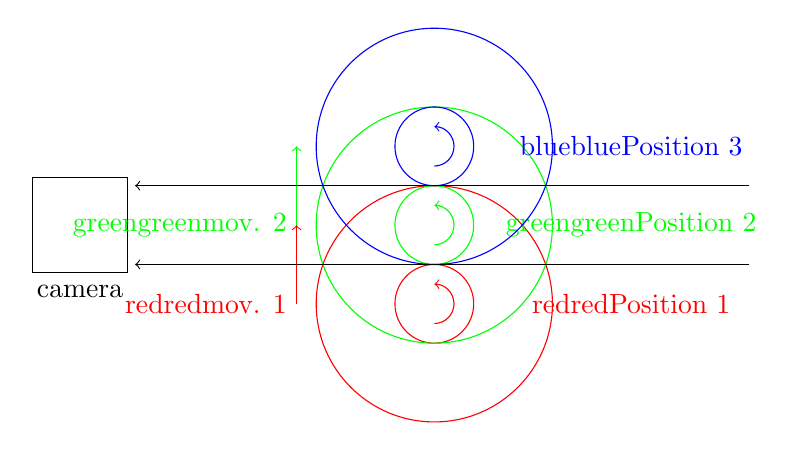
\begin{tikzpicture}
		%camera
			\draw (-.1,-.1) rectangle (1.1,1.1);
			\draw (.5,-.35) node {camera};
		% sample positions
			\foreach \x/\color in {1/red,2/green,3/blue}{
				\draw[color=\color]    (5,\x-1.5) circle (.5) circle (1.5);			
				\draw[color=\color,->] (5,\x-1.75) arc (-90:90:.25);
				\draw[color=\color]    (7.5,\x-1.5) node {Position \x};
				}
		% movement		
			\foreach \x/\e/\color in {1/3.25/red,2/3.25/green}{				
			    \draw[color=\color,->] (\e,-1.5+\x) node [left] {mov. \x} -- (\e,-.5+\x);
			    }
			 \foreach \x in {1,2}{				
		% beam
				\draw[<-] (1.2,\x-1) -- (9,\x-1);
				}
	\end{tikzpicture}
%%%%%%%%%%%%%%%%%%%%%%%%%%%%%%%%%
\end{preview}	
\end{document}
	\caption{Or is this better for the understanding?: Covering the FOV -- three scans $\rightarrow$ sample has to move, explain that we still only do \SI{180}{\degree} scans!}
	\label{fig:covering-three scans b}
\end{figure*}

To cover the desired FOV, the projection images have to be obtained in such a manner that they overlap each other slightly. This overlap is necessary for the compensation of variations in the imaging process and correct stitching of the single projections into one big projection image. 

After correction, the projections of the single overlapping subscans are merged into one projection which covers the full FOV chosen by the user (see figure~\ref{fig:merge-proj}). To achieve a correct stitching of the sub-scan projections, the cutting line to remove the overlap is calculated using the mutual difference between adjacent subscans \todo{Xris: Documentation of notch-method?}.

Since the amount of obtained projection varies for different positions of the sample in relation to the camera window---at outer positions we record more projections compared to central positions to fulfill the sampling theorem---different amounts of projections have been obtained for each subscan. If $N_x$ is the total amount of projections for each subscan we cannot simply stitch together all the images from 1 to $N$ for each subscan $x$, or we will end up with wrong merged projections. Instead, we have to stitch them together in such a way that we chose the correspondent adjacent projections. \todo{Mention potential interpolation of the inner scans?}  This has been achieved using a custom MATLAB\textsuperscript{\textregistered} script which incorporates the loading, normalizing, interpolation and correct stitching of the images into wide field projections as seem in the aforementioned figure.

After the merging of the normalized projections, the merged projections were reconstructed into the virtual tomography slices using a standard filtered backprojection algorithm or a FFT-based gridrec algorithm~\cite{Dowd2003} on a 20-node server farm (Pentium 4, 2.8 GHz processor, 512 MB RAM \todo{cluster node specs?}). This reconstruction results in an image stack of 1024 or 2048 image slices in tif-format, depending on the binnig chosen at recording time. The size of the images recorded for this publication varies from 2996$\times$2996 pixels up to 9703$\times$9703 pixels \todo{9703 px not really reconstructed up to now\ldots}.